% !TEX root = ../main.tex
% =====================================================================
% 2. BACKGROUND
%
% Everything the proposed method builds on, explained once. The notation
% table here is the ONLY place symbols are defined; later sections use
% them without re-introducing them.
% =====================================================================

\section{Background}
\label{sec:background}

% ---------------------------------------------------------------------
\subsection{Time series classification and notation}
\label{sec:bg:tsc}

A univariate time series of length $\nsteps$ is an ordered list of measurements
$\bag = (\inst_1, \dots, \inst_{\nsteps})$, and time series classification assigns to that complete
list a single label $y \in \{1, \dots, \nclz\}$. Because the value at one time step depends mostly
on its neighbours, convolutional models fit this data well, which is why the standard deep baselines
(FCN, ResNet and InceptionTime, \Cref{sec:intro:sota}) are all convolutional. All three end with
global average pooling, which averages the $\nsteps$ time steps into a single vector before the
classifier and therefore removes the per-time-step information an explanation requires. Building an
encoder that never removes that information is the object of \Cref{sec:methods:encoder}.

\Cref{tab:notation} defines the symbols used in the rest of this report. They follow
\citet{early2024millet} so that the proposed pooling heads and the baseline can be compared line by
line. These symbols are not redefined later.

\begin{table}[h]
\caption{Notation used throughout this report.}
\label{tab:notation}
\begin{center}
\small
\setlength{\tabcolsep}{5pt}
\begin{tabular}{@{}ll@{\qquad}ll@{}}
\toprule
\textbf{Symbol} & \textbf{Meaning} & \textbf{Symbol} & \textbf{Meaning} \\
\midrule
$\bag = (\inst_1,\dots,\inst_{\nsteps})$ & input series (the bag) & $\emb_j \in \R^{\dmodel}$ & embedding of time step $j$ \\
$\inst_j$          & value at time step $j$ (an instance) & $\instpred_j \in \R^{\nclz}$ & per-time-step class logits \\
$\nsteps$          & number of time steps                & $a_j$, $a_j^k$ & attention gate (shared / per class) \\
$\nclz$            & number of classes                   & $g_j^k = a_j^k \instpred_j^{\,k}$ & evidence of step $j$ for class $k$ \\
$y$                & class label of the series           & $\bagpred \in \R^{\nclz}$ & bag logits (the prediction) \\
$B$                & batch size                          & $\interp \in \R^{\nclz \times \nsteps}$ & interpretation (importance map) \\
$\dmodel$          & encoder width (channels)            & $\mathbf{h} \in \R^{\dmodel \times \nsteps}$ & feature map inside the encoder \\
$\dattn$           & attention hidden width              & $\odot$ & element-wise product \\
$\delta$           & dilation of a convolution           & $[\,\cdot\,;\,\cdot\,]$ & concatenation along channels \\
$\mathcal{K}$      & set of kernel sizes in a block      & $\sig$ & sigmoid function \\
\bottomrule
\end{tabular}
\end{center}
\end{table}

% ---------------------------------------------------------------------
\subsection{Multiple Instance Learning}
\label{sec:bg:mil}

\paragraph{Bags, instances, and weak supervision.}
Multiple Instance Learning \citep{dietterich1997mil} is a form of weakly supervised learning in
which training labels are attached to \emph{groups} of examples rather than to individual ones. A
group is a \emph{bag} and its members are \emph{instances}; the bag carries a label, the instances do
not. In the original formulation of \citet{dietterich1997mil} a molecule is a bag and each of its
possible three-dimensional shapes is an instance: the molecule is known to bind or not to bind a
receptor, but which shape is responsible is unknown. Formally, a bag
$\bag = (\inst_1, \dots, \inst_{\nsteps})$ has an observed label $y$ while the instance labels
$y_1, \dots, y_{\nsteps}$ exist conceptually but are never observed. The problem is to predict $y$
from the bag and, ideally, to recover which instances were responsible.

\paragraph{Why a time series is a bag.}
This is exactly the structure of time series classification. The series as a whole is labelled, but
in most datasets only a few time steps carry the evidence for that label: the abnormal beat in a long
recording, the spike in a traffic trace. Treating the series as the bag and each time step as one
instance turns the interpretability question into a MIL question -- recovering instance-level
contributions from a bag-level label. \Cref{fig:mil_view} shows the correspondence.

\paragraph{Pooling: how instances become a bag prediction.}
An encoder $f_\theta$ maps every instance to an embedding,
\begin{equation}
  \emb_j = f_\theta(\bag)_j \in \R^{\dmodel}, \qquad j = 1, \dots, \nsteps ,
  \label{eq:encoder_generic}
\end{equation}
and a \emph{MIL pooling function} combines the $\nsteps$ embeddings into one bag prediction
$\bagpred \in \R^{\nclz}$. The choice of pooling function distinguishes MIL methods from one another
and determines whether an interpretation can be recovered at all. The two elementary choices are
rigid: mean pooling, $\bagpred = \frac{1}{\nsteps}\sum_j W_c\emb_j$, treats every instance as equally
important and cannot single out evidence, while max pooling keeps only the strongest instance and
cannot represent evidence spread over several.

Attention-based MIL \citep{ilse2018attention} removes this rigidity by \emph{learning} how much each
instance counts. A small network scores each embedding and the scores are normalised over the bag,
\begin{equation}
  \alpha_j = \frac{\exp\!\big(\mathbf{w}^\top \tanh(W\emb_j)\big)}
                  {\sum_{i=1}^{\nsteps}\exp\!\big(\mathbf{w}^\top \tanh(W\emb_i)\big)},
  \qquad
  \bagpred = W_c \sum_{j=1}^{\nsteps} \alpha_j \emb_j ,
  \label{eq:abmil}
\end{equation}
so the bag embedding is a weighted average whose weights are produced by the model itself. Because
$\alpha_j$ is exactly the quantity used to build the prediction, it can be read directly as an
importance score for instance $j$; no separate explanation step is involved. \citet{ilse2018attention}
also propose a \emph{gated} version in which a second branch modulates the first,
$\tanh(V\emb_j) \odot \sig(U\emb_j)$, making the scoring more selective. This is the property that
\millet{} and every pooling head in this report reuse.

\paragraph{MIL beyond time series.}
The most active application of MIL is histopathology, where a whole-slide image of 40{,}000 $\times$
40{,}000 pixels is cut into thousands of patches: the slide is the bag, each patch an instance, and
only the slide-level diagnosis is known. Two methods from that literature are adapted here.
MS-DA-MIL \citep{hashimoto2020msdamil} runs the same attention-based MIL pipeline at several
magnifications and fuses the results, on the grounds that evidence appears at different scales.
DSMIL \citep{li2021dsmil} uses two streams: one aggregates all instances, the other identifies the
single most critical instance and re-weights the rest by their similarity to it, letting one decisive
instance dominate without discarding the others as max pooling would.

\begin{figure}[t]
  \centering
  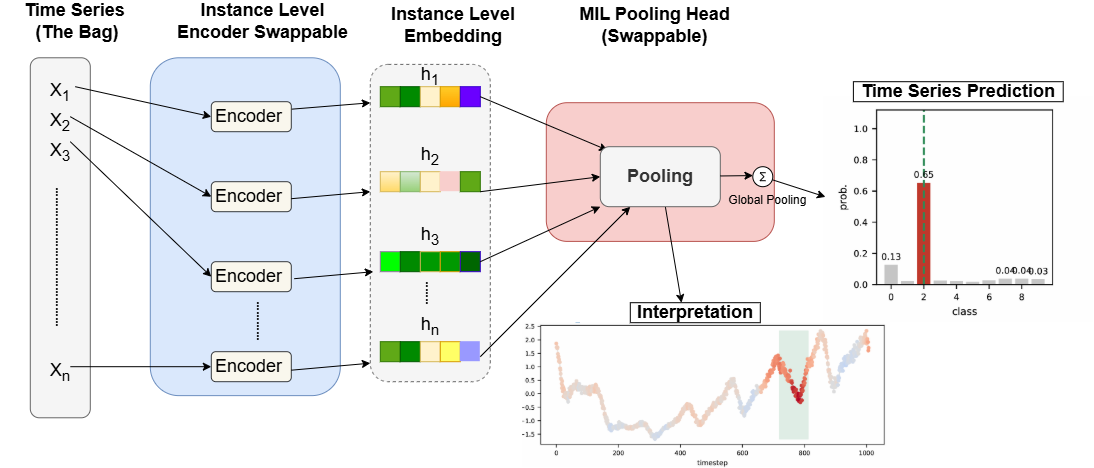
\includegraphics[width=0.90\linewidth]{figures/fig02_mil_view.png}
  \caption{The MIL view of a time series, read left to right. The series is the \emph{bag} and each
  time step $\inst_j$ is one \emph{instance}. The same encoder is applied at every time step and
  produces one instance embedding per step; the MIL pooling head weights those embeddings and
  combines them into a class prediction (right). Keeping the same weighted contributions instead of
  discarding them yields the interpretation below: one importance value per time step, drawn on the
  original series (red = pushes towards the predicted class, blue = pushes away). Both grey boxes
  are interchangeable, which is what allows any encoder of \Cref{sec:methods:encoder} to be paired
  with any pooling head of \Cref{sec:methods:pooling}.}
  \label{fig:mil_view}
\end{figure}

% ---------------------------------------------------------------------
\subsection{\millet{}: the baseline of this work}
\label{sec:bg:millet}

\begin{priorwork}
\millet{} \citep{early2024millet} is the main baseline of this internship. Everything in this
subsection is their work. I reuse their model formulation, their metric implementation and their
data loaders without modification; my only change was to wrap their code inside the pipeline of
\Cref{sec:setup:pipeline} so that their models and mine run under identical conditions. The
encoders of \Cref{sec:methods:encoder} and the pooling heads of \Cref{sec:methods:pooling} are my
own work and are written in the notation used here, so the two can be compared directly.
\end{priorwork}

\millet{} applies the MIL view of \Cref{sec:bg:mil} to time series classification. An InceptionTime
encoder produces one embedding per time step as in \Cref{eq:encoder_generic}, and a MIL pooling head
turns those embeddings into a bag prediction $\bagpred$ together with an interpretation
$\interp \in \R^{\nclz \times \nsteps}$, where $\interp_{k,j}$ quantifies how much time step $j$
pushed the model towards class $k$. Their best head, \emph{conjunctive pooling}, combines a single
attention gate with a per-time-step classifier:
\begin{align}
  a_j       &= \sig\!\left(\mathbf{w}_a^\top \tanh(W_a \emb_j)\right) \in [0,1],
  \label{eq:conj_gate}\\
  \instpred_j &= W_c \emb_j + \mathbf{b}_c \in \R^{\nclz},
  \label{eq:conj_inst}\\
  \bagpred^{\,k} &= \frac{1}{\nsteps} \sum_{j=1}^{\nsteps} a_j\, \instpred_j^{\,k},
  \qquad
  \interp_{k,j} = a_j\, \instpred_j^{\,k}.
  \label{eq:conj_bag}
\end{align}
The gate $a_j$ decides how much weight time step $j$ receives and the classifier $\instpred_j$
decides what it argues for, and \Cref{eq:conj_bag} builds the class score as the average over time
of the vote weighted by the attention. The essential property is that $\interp_{k,j}$ consists of the
same terms that are summed to produce $\bagpred^{\,k}$: the explanation cannot disagree with the
prediction, because it is the prediction, decomposed.

\paragraph{Limitations of conjunctive pooling.}
Three properties of \Cref{eq:conj_gate}--\Cref{eq:conj_bag} restrict what the head can express.
Each one motivates a corresponding family of pooling heads in \Cref{sec:methods:pooling}, which are
presented in the same order and each labelled with the limitation it addresses.

\begin{enumerate}\itemsep3pt
  \item[\textbf{L1}] \textbf{A single attention gate is shared across classes.} The gate $a_j$ in
        \Cref{eq:conj_gate} is one scalar per time step, used unchanged for all $\nclz$ classes.
        Consequently the head cannot represent a time step whose evidence is class-dependent -- one
        that is highly relevant to one class and irrelevant to another -- because a single value
        must serve every class simultaneously.
  \item[\textbf{L2}] \textbf{The attention weights are not normalised over time.} The gate is a
        sigmoid, so the weights lie in $[0,1]$ individually but do not sum to a fixed quantity, and
        the aggregation divides by $\nsteps$. The magnitude of $\bagpred^{\,k}$ therefore depends on
        the length of the series: two series carrying identical evidence but of different lengths do
        not receive comparable scores. This is a practical concern on the \ucr{} archive, whose
        series lengths range from 15 to 2{,}844.
  \item[\textbf{L3}] \textbf{The aggregation is a fixed mean, so evidence is diluted on long
        series.} \Cref{eq:conj_bag} averages over all $\nsteps$ time steps with equal weight, and
        this operator is fixed rather than learned. When the evidence is concentrated in a few
        decisive time steps and the series is long, those steps contribute a vanishing share of the
        mean and are diluted by the surrounding background. The mean has no mechanism to counteract
        this, and no ability to adapt to datasets where the evidence is instead spread out.
\end{enumerate}

% ---------------------------------------------------------------------
\subsection{Measuring the quality of an explanation}
\label{sec:bg:metrics}

An importance map can look convincing and still be wrong, so explanation quality has to be measured.
This report uses the two metrics of \citet{early2024millet}, computed with their implementation.

\paragraph{AOPCR: faithfulness of the explanation to the model.}
The Area Over the Perturbation Curve \citep{samek2017aopc} tests whether the time steps an
explanation calls important are the ones the model relies on. The steps are ranked from most to least
important according to the model's own interpretation, masked one at a time in that order, and the
confidence in the original prediction is tracked as masking proceeds; a faithful explanation produces
a fast drop. Writing $\bagpred^{k}(\bag)$ for the confidence in class $k$, $O^k$ for the ranking
induced by $\interp_{k,\cdot}$, and $\bag^{O^k}_{j}$ for the series with its $j$ most important steps
masked,
\begin{equation}
  \text{AOPC}(\bag, O^k) \;=\; \frac{1}{\nsteps-1}\sum_{j=1}^{\nsteps-1}
  \Big[\bagpred^{k}(\bag) - \bagpred^{k}\big(\bag^{O^k}_{j}\big)\Big] .
  \label{eq:aopc}
\end{equation}
AOPC on its own would reward a model whose confidence is simply fragile, so \citet{early2024millet}
add a random control. AOPCR repeats \Cref{eq:aopc} with three random orderings
$R^{(1)}, R^{(2)}, R^{(3)}$ and reports the margin of the real ranking over chance:
\begin{equation}
  \text{AOPCR}(\bag, O^k) \;=\; \frac{1}{3}\sum_{r=1}^{3}
  \Big[\text{AOPC}(\bag, O^k) - \text{AOPC}\big(\bag, R^{(r)}\big)\Big] .
  \label{eq:aopcr}
\end{equation}
A higher AOPCR means the ranking identifies evidence rather than noise. AOPCR needs no
per-time-step ground truth, so it can be computed on every dataset in this study. One property
governs how it may be used: it is built from raw confidence differences, so its scale follows the
scale of the model's logits and has no fixed range. AOPCR values are comparable across models trained
under an identical configuration, but not against AOPCR values reported elsewhere for models trained
differently -- \Cref{sec:disc:reading} gives direct measured evidence of this.

\paragraph{NDCG@$n$: ranking quality of the explanation against ground truth.}
The Normalised Discounted Cumulative Gain \citep{jarvelin2002ndcg} answers a different question: do
the time steps that genuinely matter appear at the top of the ranking? That requires knowing which
steps genuinely matter, which is available only for \webtraffic{}, where the generator records which
steps it modified to create each class. Writing $\text{rel}_j \in \{0,1\}$ for whether the step
ranked $j$-th is one of the modified steps,
\begin{equation}
  \text{NDCG@}n(O^k) \;=\; \frac{1}{\text{IDCG@}n}\sum_{j=1}^{n}
  \frac{\text{rel}_j}{\log_2(j+1)} ,
  \label{eq:ndcg}
\end{equation}
where $\text{IDCG@}n$ is the same sum evaluated on the ideal ranking. The normalisation gives
$\text{NDCG@}n \in [0,1]$, with $1.0$ for a perfect ranking.

The two metrics are complementary. AOPCR measures \emph{faithfulness} -- agreement between the
explanation and the model's own behaviour -- and is available on all datasets but is unnormalised.
NDCG@$n$ measures \emph{correctness} against an external ground truth and is normalised, but can
only be computed on \webtraffic{}. Where the two disagree, NDCG@$n$ is the stronger evidence,
because it is checked against a known answer.
